\section{Routing protocols from local spectral prices}\label{sec:protocol}

Fix a finite field $F$ with largest spectral flat dimension $k$.
Given a permutation of $n=2^h$ records, we seek an exact identity
for its payload matching together with a fixed set of catalyst wires.
Place opposite ends of a catalyst at $-Me_j$ and $Me_j$ on a spectral
$k$-flat, at distance $M$ from the origin. Its price is $2M$ per bit.
For $N_c$ such bits and payloads of width $w$, returning the catalysts
along these segments costs $2MN_c/w$ units of the budget in \eqref{eq:protocol-budget}. The protocol allows a further
$10n$ units in each term of the exact identity.

There are two charges for a link. Installing $yw$ bits on a link of
length $\lambda$ costs $\lambda y$, and using a pair of slots at
address scale $t$ costs $t^p$. At positive scale $\lambda=1$, and
one slot has at most $2^{th+o(h)}$ possible partners. In
Section~\ref{sec:width}, terms that spend too little on the
catalysts contribute an error with a price gap. In the surviving
terms the excess budget limits both the payload width routed at
positive scale and the number of slot pairs that carry it. For
example, at scale $t$ it leaves capacity for at most $O(n/t^p)$ chunks of width $t^p w$
with a constant independent of $t$ (Lemma~\ref{lem:tag-shorter}).
The local tables may depend on the fixed scales. For the later
application, $w$ grows polynomially faster than $h$, so specifying
the local choices takes $o(nw)$ bits.

\begin{definition}[Multidirectional routing protocol]\label{def:protocol}
Fix real parameters
\[
 A>1,\qquad p>1,\qquad T_0=2^{-W}\text{ for a positive integer $W$}.
\]
Write \(n=2^h\). For all sufficiently large integers \(h\) and every integer
\(h\le w\le h^A\), the protocol has the following properties, uniformly in
\(h,w\) and the permutation. All constant bounds and finite menus may depend
on the fixed parameters and on \(F,k\).
\begin{enumerate}
\item Give each of \(O(n)\) sites a fixed layer coordinate. The available
layers are \(0\) and \(\pm M e_j\) for \(1\le j\le k\), with \(M>1\) a fixed integer.
The payload ports encode two lists of \(n\) records of width \(w\) in layer
zero. Each of \(N_c=O(nw)\) catalyst bits is paired from \(-M e_j\) to
\(+M e_j\) for an assigned direction \(j\). Each site has \(O(w)\) external
bits. These assignments are independent of the tags and all selectors.
For any valid permutation tags, the tensor of the prescribed payload
matching times these catalyst identities equals an ordinary sum over \(F\)
of the terms below.
\item A deterministic control reads the tags and the selector.
The selector has \(O(nh\,\operatorname{polylog}h)\) bits. The control rejects
invalid selectors and describes one term per accepted selector. It is an advised RAM with
\(O(h)\)-bit words, \(O(n\,\operatorname{polylog} h)\) word steps, and the
same bound on the numbers of input, output, memory, and advice words. Each
step acts on a bounded number of registers and accessed words, including
its address computation and next control state, by a Boolean circuit of
size \(O(h\,\operatorname{polylog}h)\) apart from memory selection (a fixed circuit for each time step, regardless of transcript).
\item A term installs equality links between communication slots and a
local tensor at each site. Each site has a fixed bounded number of slots of
capacity \(O(w)\) bits, with a fixed ordering of their bits. A fixed
partition of all slots into groups prescribes the permitted links.
A slot belongs to at most one installed link in a term, and the two
slots of a link belong to the same group. A group has scale \(t=0\) or
\(t=T_0\). Its cardinality is
\(O(1)\) at scale zero and at most \(2^{th+o(h)}\) at positive scale.
A link has integer width \(yw\) and length charge \(\lambda\) from a
fixed finite set of nonnegative rationals. A link between different
layers has scale zero and charge at least the Euclidean distance between
the layers. At positive scale, \(\lambda=1\).
Each local tensor has a fixed trivalent implementation of size
\(O(w\,\operatorname{polylog}h)\), on a fixed topology configured only by setting
\(O(h\,\operatorname{polylog}h)\) inputs from the control.
The port positions include padding. Unused bits can be pinned to zero.
\item Every accepted term obeys
\begin{equation}\label{eq:protocol-budget}
  \sum_{\text{links}}\bigl(\lambda y+t^p\bigr)
          \le 10n+\frac{2M N_c}{w}.
\end{equation}
\end{enumerate}
\end{definition}

\begin{theorem}[Routing under a maximal flat dimension]\label{thm:protocol}
Let $F$ be a finite field whose largest spectral flat has dimension $k$.
For every real $A>1$, every rational $p>1$, and all sufficiently large
integers $W$ with $pW$ integral, there is a multidirectional routing
protocol as in Definition~\ref{def:protocol}.
\end{theorem}

The construction has two steps. First we give a criterion for building
such an identity. A local spectral price test can justify replacing a
set of wire demands by a cheaper sum of alternatives. If prices instead
pass the tests, the criterion allows us to add links, called
\emph{probes}, provided the resulting change in prices pays their
capacity fees. The tests ask whether a bounded neighborhood admits
particular wire prices. For the finite precision used by the control,
the answers and the required exact replacement identities can be
recorded in finite tables. We then construct a layout and a choice of probes that
satisfy the criterion. This second step uses the exclusion of Euclidean
$(k+1)$-cubes under the maximal-flat hypothesis.

\subsection{Adaptive probing with several catalysts per column}

Fix a permutation and a layout with $O(n)$ columns. Each column has a center and $2k$ ends, with a
catalyst pair between the two ends in each direction. The available
\emph{core} links form a graph of bounded degree. They include a link of
length $M$ and scale zero from the center to each end. Thus each catalyst
pair has a route of cost $2M$ per bit. The column layout is fixed independently of the permutation. One \emph{activation} selects a
further bounded-degree list of links, its \emph{probes}. Core and probe
links obey the slot, scale and length conditions in
Definition~\ref{def:protocol}. Reserve separate slots for the core and
for each purchase of an activation. Write their normalized capacity fees as
\[
 P_{\mathrm{core}}=\frac{1}{n}\sum_{\mathrm{core}}t_e^p
 \le1,\qquad P=\frac{1}{n}\sum_{\mathrm{probes}}t_e^p.
\]
Once an edge is available, installing $b$ bits on it incurs the further
linear cost $b\lambda_e/(nw)$.

A \emph{commodity} $i$ is an indexed pair of sites, with a prescribed
bounded-hop core route of total length at most $a_i$. The bounds $a_i$
belong to a fixed finite set of positive rationals. There are $O(n)$
commodities of bounded incidence, including a distinct commodity for
each of the $n$ payload demands. Repetitions of pairs are permitted.
Fix the column, payload and slot layouts as in Definition~\ref{def:protocol}.
Each slot may have capacity a fixed constant times $w$, and slots may be
replicated for boundedly many purchases. The control must compute
all layouts, routes and lists within its prescribed bounds. All constants
are independent of $h,w$ and the permutation.

For each commodity $i$, keep an inventory of outstanding bits. The
first demands enter this inventory as payloads requested between paired
sites. Replacing a
demand by a tensor identity can consume some of them and create new
demands. Any remaining bit on commodity $i$ can always be routed along
the core for at most $a_i/(nw)$ in our normalized budget.

Assign each commodity a provisional price $x_i\in[0,a_i]$. These
numbers record marginal costs of the inventory. The following test
asks whether one spectral price system agrees with them on a prescribed
neighborhood. Write $[0,a]$ for the box of provisional prices.
At every site take a ball of fixed radius in the undirected core.
For all pairs with both endpoints in the ball require a spectral price
system over $F$ to realize the commodity prices $x_i$, to give each
catalyst pair price $2M$, and to give each core link price at most its
length. When testing a purchased activation impose the last inequality
also on its probes. The discrepancy of the ball is the least maximum
of the absolute errors in the equalities and the positive violations of
the inequalities. Allow zero scale. The zero price bounds the minimum
from above, and the length bounds on a spanning tree of the ball then
bound the scale of a minimizing sequence. Compactness of the normalized
spectrum gives attainment. A singleton has the zero wire metric.
A sequence of arrays, with $h\to\infty$, is \emph{consistent} for the
specified test if the discrepancy summed over all roots and divided by
$n$ tends to zero. The local price systems at different roots may vary.
A ball discrepancy is $1$-Lipschitz for the maximum norm on its price
coordinates. Bounded overlap consequently gives uniform continuity of
the mean discrepancy in the normalized Euclidean norm. At fixed
precision a finite table for each of finitely many local formats implements
the discrepancy test with any required fixed slack.

A failed test permits a local tensor identity in which every summand
costs strictly less than the demands it replaces. To realize that saving
there must be enough outstanding bits on the commodities with positive
price. We therefore determine the provisional prices from the inventory.

Use the inner product $\langle u,v\rangle=n^{-1}\sum_i u_iv_i$.
The layout supplies a score $f$ on the box with $f(0)=0$, uniformly
strongly convex, with uniformly Lipschitz gradient and uniformly bounded
gradient coordinates. Require $\nabla_i f(x)=0$ when $x_i=0$.
If $z$ is the inventory (outstanding commodity widths in units of $w$), define, for $0<s\le1$,
\[
 F_s(z)=\max_{0\le x\le a}\{\langle z,x\rangle-sf(x)\},\qquad
 x_s(z)=\mathop{\rm argmax}_{0\le x\le a}
          \{\langle z,x\rangle-sf(x)\}.
\]
The components of $x_s(z)$ are the marginal costs of adding inventory
to $F_s$. Strong convexity and the lower-face gradient condition ensure that
positive marginal prices occur only on commodities with positive stock.
As $s$ decreases to zero, $F_s(z)$ tends to $\langle a,z\rangle$,
the upper bound obtained by routing every demand along the core.

For each fixed rational $s$, the control must evaluate $f$ to $o(1)$
on a vanishing-mesh grid of $O(\log h)$ bits per coordinate. On every
coordinatewise bounded inventory $z\ge0$ on the $1/w$ mesh it must
return a grid approximation to $x_s(z)$ with $o(1)$ error in normalized
norm. These convergence hypotheses are uniform in the permutation and the
remaining variable parameters, along every subsequence of $h$. Choose a
continuous function $j:(0,1]\to[0,\infty)$ with integral at most one. Define the excess of $x$ at $s$ to be $f(x)-j(s)$, taking its
maximum with $n^{-1}\sum_{i\ {\rm payload}}x_i-1$ at $s=1$.

\begin{proposition}[Multidirectional adaptive probing]
\label{prop:adaptive-probing}
Suppose that for each fixed rational $0<s\le1$ the control can choose
an activation from a grid array $x$. Suppose that for every
core-consistent sequence of grid arrays with strictly positive lower
limit of the excess, and every sequence $x'$ consistent with the
resulting activations, one has
\begin{equation}\label{eq:protocol-activation}
 \liminf_{h\to\infty}
 \left(\frac{s}{2}\mathcal D_f(x',x)-P\right)>0,\qquad
 \mathcal D_f(y,x)=f(y)-f(x)-\langle\nabla f(x),y-x\rangle .
\end{equation}
Then the layout admits the protocol of Definition~\ref{def:protocol}.
Each column has $O(w)$ bit wires for each pair of opposite ends,
with $N_c=O(nw)$ such wires in total. Their locations are fixed
independently of the permutation and the selector.
\end{proposition}

\phantomsection\label{app:probing-proof}
\begin{proof}
Fix a summand. Write $wz_i$ for its outstanding bits on commodity $i$.
Record the bit positions in order at each endpoint, so any subsequent
identity on these positions is valid under the surrounding contractions.
Let $S$ count the normalized capacity fees and linear costs already
incurred, less a credit of $2M/(nw)$ for each external catalyst bit
used in a replacement. An unused catalyst bit can be routed through
its column center for exactly its credit. Thus, once all commodity
demands are met, the total cost is at most $S+2MN_c/(nw)$. We control
the cost of unfinished demands by the potential $F_s(z)$.

\paragraph{Marginal cost of a demand.}
Let $\mu$ be the strong convexity constant of $f$. At the maximizer
$x=x_s(z)$ the box optimality condition gives
\[
                        z_i\ge s\nabla_i f(x)\ge s\mu x_i .
\]
For the second inequality, vary only coordinate $i$ and use the
vanishing of $\nabla_i f$ on its lower face. On that face the first
inequality follows from $z_i\ge0$. In particular, a price bounded away
from zero guarantees stock when $s$ is bounded away from zero. Choose
an integer $B$ greater than every gradient coordinate bound. For
$z_i\ge B$ we have $x_i=a_i$. We can therefore fulfill all stock above
$B$ along the prescribed route at cost at most $a_i/n$ per unit while
decreasing $F_s$ by precisely that amount per unit. We apply this cap
after every stock increase.

With the inventory norm induced by $\langle\cdot,\cdot\rangle$, the
two optimality inequalities and strong convexity give
\[
 \|x_s(z)-x_{s'}(z')\|
       \le \frac{\|z-z'\|+C|s-s'|}{\mu\min(s,s')}.
\]
Comparing the two maxima at their respective optimizers now gives
$\nabla_z F_s(z)=x_s(z)$ and $\partial_s F_s(z)=-f(x_s(z))$.
For bounded inventories and $s,s'$ in a compact subinterval of
$(0,1]$, the preceding estimate makes the first-order remainder
uniformly quadratic. We will use these derivatives both to price a
local replacement and to pay for new probes.

\paragraph{A failed test gives a cheaper exact identity.}
On a ball that fails the test, demand one bit of each positive-priced
commodity and of every catalyst pair. Let $L$ be the sum of their
assigned prices. The zero wire metric fails the test, so $L>0$.
Available replacements are commodities at prices $x_i$, catalyst pairs
at $2M$, and core links and currently tested probes at their lengths
$\lambda_e$. A replacement commodity enters the inventory. A
replacement catalyst pair can be installed immediately along its center
route.

Increase all replacement prices by the same sufficiently small amount
to obtain positive lengths $l_e$. On a nonsingleton ball, every
normalized spectral wire metric $d$ then satisfies
\[
             \sum_{e\ \mathrm{demanded}}d_e
               < L\max_{e\ \mathrm{available}}d_e/l_e .
\]
The connected core makes the maximum positive. If no increase works, take a
sequence of violations as the price increase tends to zero and rescale
each violating metric to make its maximum ratio one. The lengths of
a spanning tree bound the scales. In the limit every replacement
respects its original price bound, yet the sum of the demand distances
is at least $L$. Each demand must therefore attain its own bound.
This realizes the prices of all catalysts and positive-priced commodities,
and the zero-priced commodities have distance zero. The resulting metric
passes the test, a contradiction. On a singleton all demands can be
supplied locally.

By compactness the displayed inequality holds with some $L_-<L$ in
place of $L$. Take the product of width-$b_0$ demand wires. As supply,
take the direct sum over replacement options $e$ of a single wire of
width $\lfloor b_0 L_-/l_e\rfloor$ on $e$. For large fixed $b_0$ every
spectral point values the supply strictly above the demand, by the
uniform margin. Lemma~\ref{lem:spectral-comparison} supplies the $r$th
demand power from a direct sum of at most $C(b_0)$ copies of the $r$th
supply power. Expansion gives an ordinary sum over $F$ of restrictions
of replacement products. With $b=b_0r$ bits per demand and $m$
replacement options, each term costs at most $bL_-$, and there are at
most $C(b_0)m^r$ terms. Choosing first $b_0$ and then $r$ makes the
number of bits specifying a term arbitrarily small relative to $b$.

For $J=O(w)$ simultaneous copies, the outer selector records only the
histogram of the $J$ choices. It uses $O(\log(2w))$ bits because the
alphabet is fixed. Inside that summand, transmit the full choice word
on a core spanning tree, check its histogram, and sum over the words with
that histogram. The histogram fixes the installed widths, while each word
specifies offsets within them. In this way every original word
contributes its tensor with its original coefficient. The tree has
bounded total length, so the rate just obtained makes the cost of
transmitting the word less than half the saving $Jb(L-L_-)$. Fixed
tables, prefix sums and sorting of bit positions implement the local
operations with $O(w\,\mathrm{polylog}(h))$ trivalent gates since
$w\le h^A$. Each auxiliary deterministic check has a unique valid
history.

Suppose the mean discrepancy exceeds a fixed tolerance. Bounded overlap
and bounded discrepancies yield $\Omega(n)$ disjoint balls failing by
a fixed amount. In each bounded local format the vectors whose
discrepancy reaches this fixed lower bound form a compact set. At any one
vector the saving from its identity persists on a neighborhood where every selected
positive-priced commodity stays bounded away from zero. A finite
subcover gives a fixed menu with uniform margins. An $o(1)$
normalized-norm error in the grid approximation affects only $o(n)$
balls by more than a fixed coordinate tolerance.

Use $J=\lfloor\alpha w/b\rfloor$ copies on each selected ball, checking
the actual stock and skipping deficient balls. For fixed sufficiently
small $\alpha>0$ the stock inequality at the beginning of the proof
guarantees adequate inventory on every accurate ball while $s$ stays
bounded away from zero. The $o(n)$ inaccurate balls have bounded
cost per ball in units of $w$. In this simultaneous round, use the marginal prices $x_i$ for newly
created and fulfilled demands. Include the linear link costs and deduct
the $2M$ credit for each consumed external catalyst bit. After division by $nw$ these changes decrease the
first-order estimate for $S+F_s(z)$ by at least $c\alpha$, uniformly
for large $h$. The change in inventory has normalized norm $O(\alpha)$,
so its quadratic error is $O(\alpha^2)$. Fixing $\alpha$ sufficiently
small leaves a uniform positive decrease in every new summand. This
applies to both the core test and the test with one purchased activation.

\paragraph{Paying for probes when the core test passes.}
Fix rational $s$. Suppose the excess of $x=x_s(z)$ exceeds $1/4$ and
its core discrepancy is sufficiently small. Choose the activation
from the grid approximation to $x$. For some fixed $\zeta>0$ and
test tolerance, every $x'$ of at most this discrepancy with the
purchased probes satisfies, for all sufficiently large $h$,
\[
                      (s/2)\mathcal D_f(x',x)\ge P+\zeta .
\]
If such constants did not exist, a sequence with discrepancies tending
to zero and margins tending to zero or less would contradict
\eqref{eq:protocol-activation}. Bounded coordinates and gradients,
the Lipschitz gradient, and the normalized-norm approximation let us
use the actual maximizer in the inequality.

Buy the probes once. Hold half the inventory in reserve and start with
$z/2$ at time $s/2$. The potential is then $F_{s/2}(z/2)=F_s(z)/2$.
Feeding the reserve back at rate $z/s$ as time advances to $s$ would
keep $x$ fixed and restore the original potential in the absence of
replacements. Feed at this same rate on a fine fixed rational mesh.
Before each increment, apply rounds of simultaneous local replacements
until the current maximizer $x'$ has small discrepancy with the probes.
Along the feed the instantaneous increase in potential is at most
\[
 \langle z/s,x'\rangle-f(x')
 \le F_s(z)/s-\mathcal D_f(x',x)
 \le F_s(z)/s-2(P+\zeta)/s .
\]
The first inequality is the box optimality condition
$\langle z/s-\nabla f(x),x'-x\rangle\le0$ at the original maximizer.
Over the interval of length $s/2$, the feed therefore recovers at
most $F_s(z)/2-P-\zeta$. This pays the capacity fee $P$ and decreases
$S+F_s$ by $\zeta$. The sum of the quadratic mesh errors is proportional
to the mesh spacing. Rounding the split and the increments to whole bits,
returning the original reserve exactly, costs $o(1)$. A fine enough
mesh leaves a saving of at least $\zeta/2$.

The number of replacement rounds in a purchase can be bounded uniformly
even when $S$ is negative. The stock cap and bounded derivatives give
a bound for the total possible increase from the purchase, feed and
time changes without the test. Once the accumulated replacement savings
exceed that bound plus the required saving, complete the feed directly.

\paragraph{Finishing the payloads within budget.}
Start at $z=0$, $s=1$ and pay $P_{\mathrm{core}}\le1$. On a fine fixed
mesh, inject a total of exactly $w$ bits on each payload commodity.
Next decrease time to a fixed rational $s_0>0$ with $s_0f(a)<1$
uniformly. Before each increment, bring the excess down to at most
$1/2$. Apply a replacement round at large discrepancy, or buy probes
at small discrepancy when the excess exceeds $1/4$. The overlap of
these excess thresholds allows fixed-precision decisions. Purchased
links stay paid. To choose a new activation we test the core alone.
During the corresponding feed we test the core with its new probes.

At excess at most $1/2$, the mean payload price is at most $3/2$
during injection. During the time decrease, $f(x_s(z))\le j(s)+1/2$.
Since $\int_0^1 j(s)\,ds\le1$, each phase costs at most two on a fine
enough fixed mesh, including rounding. Finally route the remaining
requests along their prescribed core routes. Substituting $a$ in the
maximum defining $F_{s_0}(z)$ shows that this costs at most
$F_{s_0}(z)+s_0f(a)$, so the final $S$ is less than $10$.

As in the purchase step, the outer loop has a uniform stopping bound.
Even without the low-excess tests, the bounded derivatives control the
sum of all injection and time-change increases, and routing capped
stock directly has bounded cost. If the accumulated decreases exceed
this crude bound, complete the scheduled injections, time changes and
routing directly. Each trajectory thus performs uniformly bounded
numbers of reductions, purchases and replacement rounds.

Reserve $O(w)$ external bits per catalyst pair in advance and return
unused bits on their center routes. Aggregate repeated uses of each
available link into a single installed width with one capacity fee.
Bounded incidence and bounded routes give a bounded number of pieces
per site and step. Widths, boundaries and histograms require
$\mathrm{polylog}(h)$ bits per piece, with $O(h)$ more bits for site
identifiers. In the fixed local topology, pad each list to its maximum
length and sort position tags to split, concatenate or permute its
pieces. This takes $O(w\,\mathrm{polylog}(h))$ gates per site. Given
the layout, value and activation routines, the control handles the
fixed-precision menus, greedy disjoint-ball packings, stock checks,
histograms and link-width lists in $O(n\,\mathrm{polylog}(h))$ word
operations. Tolerance decisions have fixed slack, so their constants
may be hardwired. Mesh arithmetic uses rationals and rounded bit counts.

Use a unique encoding for each histogram and set unused selector fields
to zero. Each replacement is an exact identity under every contraction
on its ordered bit positions. Expanding the successive replacements
therefore gives exactly the payload matching times the external catalyst
identities with the prescribed multiplicities. The normalized cost is
at most $10+2MN_c/(nw)$ in every summand, as claimed.
\end{proof}


\subsection{The routing layout}

A long wire can measure a short move in a specified direction.
In a Euclidean frame, let a record move from \(b\) to \(c=b+u\)
with \(\|u\|\le1\), and attach an end to \(c\) at distance \(M\) in the
unit direction \(\alpha\). The distance from \(b\) to this end, minus
\(M\), reads \(\langle u,\alpha\rangle+O(M^{-1})\).
The maximality of \(k\) will force this same measurement in the local
price test on a chain of moves. Along that chain, a common signed
coordinate adds. If the measured displacements of its \(H\) moves
all exceed \(\tau>0\), the endpoint distance is at least \(H\tau\), up
to the measurement errors. For \(H\tau>1\) with sufficient margin,
purchasing a link of length one between the endpoints forces at least
one measured displacement to decrease. We choose the chain length and
the link fee so that this decrease, measured by a convex score, pays
for the link with a strict surplus.

Subdividing the payload matching supplies short moves with small capacity
fees. Each position in a move receives a column whose catalyst pairs
measure its displacement. Within each group of positions, a fixed
sparse graph lets us join moves at zero charge. A probe will connect the
ends of a chain of these moves.

\paragraph{Stages and tiles.}\label{app:two}
A \emph{stage of scale $t$}, for fixed $0<t\leq 1$, has a fixed collection
of groups.  Each group has an input list and an output list of the same
length $2^{th+O(1)}$, and the lists have $O(n)$ positions in total.  A
stage specifies $n$ matched input--output pairs, with both positions in
the same group and with each position used at most once on its side.
We call each matched pair a \emph{tile}.  A permutation on $n$ positions
is a stage of scale one with a single group.


The construction groups positions by successive colors. A recursive
permutation network uses a related decomposition \cite{Benes}. Here
the control must also compute the route in linear word time on every
input matching.

\par\Needspace{4\baselineskip}
\begin{lemma}[Subdivision of a stage]\label{lem:subdivision}
Fix $0<t\leq 1$ and an integer $d\geq2$, and put $K=18(d-1)+1$.
For all sufficiently large $h$, a stage of scale $t$ can be replaced by
$K$ successive stages of scale $t/d$.  Each parent tile is routed from
its input to its output along one tile of every child stage, within the
original parent group.  At each of the $K+1$ boundaries between moves,
including the two ends, different parent tiles occupy distinct positions.
The child groups and the identifications between successive position
lists are fixed independently of the matching.  Given the matching, the
control computes the child tiles in $O(n)$ operations on $O(h)$-bit
words, with $O(n)$ words of advice and working storage.  The constants
may depend on $t,d$ and on the size bounds for the parent groups.
\end{lemma}

\begin{proof}
Put $D=2^{\lfloor th/(9d)\rfloor}$ and $L_b=D^9$.  Inside one parent
group, begin with the given pair of lists.  To split a pair of lists of
length $m_1$, partition each list into blocks of $L_b$ positions, padding
the last block.  Color every matched pair with one of $D$ colors so that
at either endpoint at most $4D^8$ pairs of its color use its block.
For a greedy assignment, a block with $4D^8$ previous pairs of one color
forbids that color.  Each endpoint block forbids at most
$L_b/(4D^8)=D/4$ colors, so a color is always available at both ends.
We give the time bound for the assignment below.

In each block reserve $4D^8$ positions for every color, in a fixed order.
One entering stage sends each occupied input position to the next free
position of its color in the same block.  One exiting stage sends the
corresponding color positions on the output side to their final
positions.  Allocate the output-side positions in the same processing
order, using a separate counter for each block and color.  Both stages
use groups with $4L_b$ positions on each side after padding.  Between
them there remains, for each color, a matching between its positions
across all blocks.  Its two lists each have length
\[
        m_2=4D^8\lceil m_1/L_b\rceil.
\]
The fixed relabeling by color and block identifies each position of an
entering or exiting stage with a unique position of the intervening lists.

Repeat this operation on each remaining list pair for $q=9(d-1)$ rounds.
Starting from $m_0=2^{th+O(1)}=\Theta(D^{9d})$, the length after $j$
rounds is $\Theta(D^{9d-j})$ for $0\leq j\leq q$.  Indeed, before
the last split the length is at least a constant times $D^{10}$, and
each split of a list of length $m_1\geq L_b$ gives
$4m_1/D\leq m_2\leq8m_1/D$.  Thus every final list has length
$\Theta(D^9)=2^{th/d+O(1)}$ and supports one central stage.  Reading
the $q$ entering stages, the central stage, and the $q$ exiting stages
in reverse nesting order gives the asserted $K$ moves.  In one round
the $D$ separated lists together have length at most $8m_1$.  Since the
number of rounds is fixed, each phase inside the parent group has
$O(m_0)$ positions and can be padded to a common length
$\Theta(m_0)$.  Each matched pair uses distinct endpoints at each step
by its allocated positions and the inductive matching property.

It remains to assign colors in linear time.  Let $\ell=\lceil Ch\rceil$
for an absolute constant $C$.  Hardwire $D^4$ strings of $\ell$ colors
so that, for every $S\subseteq\{1,\ldots,D\}$ of size at most $D/4$,
fewer than $D$ strings have at least half their entries in $S$.
To obtain the strings, sample their entries independently and uniformly.
For fixed $S$ the probability for one string is $\exp(-\Omega(\ell))$.
The probability of failure for some $S$ and some $D$ strings is at most
$2^D\binom{D^4}{D}\exp(-\Omega(\ell D))<1$ for sufficiently large $C$,
since $\log D\leq h$.

For each block store a bit mask for each string.  A bit is set when the
corresponding color is forbidden in this block.  When a color first
becomes forbidden, set its bits using the list of its occurrences across
the strings.  Initialization and all such updates cost $O(D^4\ell)$
word operations per block.  For a matched pair with within-block
positions $u,v$, try the string indexed by
$(u\bmod D^2,v\bmod D^2)$.  Take the union of its two endpoint masks.
If there is a free bit, use its color.  This takes constant time on
$O(h)$-bit words.  For example, divide a mask into a constant number of
chunks of at most $h/2$ bits and use a shared table of $O(2^{h/2})$
words to find the first free bit in a chunk.

If both masks together cover the string, scan all $D$ colors to find a
common available one.  Charge this scan to an endpoint block whose mask
covers at least half the string.  Its final set of forbidden colors has
size at most $D/4$.  By the choice of strings, fewer than $D$ strings
can receive charges at that block.  A fixed string is tried there at
most $L_b/D^2=D^7$ times, since it fixes the residue of the position
on that side and the matching uses each position at most once.  Thus all
scans charged to a block cost at most $D\cdot D\cdot D^7=L_b$ word
operations.  Also $D^4\ell=O(L_b)$ for fixed $t,d$ and sufficiently
large $h$.  Summing over the blocks in the fixed number of rounds proves
the claimed bounds.  Fixing the order of the pairs and taking the first
available color in either search makes the routing deterministic.

The scans, shifts, comparisons and table reads used here fit
Definition~\ref{def:protocol}. If a word operation needs multiplication
by an advice-fixed constant, split the operands into a bounded number of
pieces of at most $h/3$ bits. A shared product table of $O(2^{2h/3})$
words and a bounded number of additions and shifts suffice.
\end{proof}


\paragraph{Columns and links.}
Fix the parameters in Definition~\ref{def:protocol}. Choose a large
integer \(W\) and set
\[
       t=2^{-W},\qquad T=t^2,\qquad H=\lceil 32 k/T\rceil .
\]
In this section \(H\) denotes a chain length. Apply Lemma~\ref{lem:subdivision} to the one-stage permutation with
subdivision factor $1/t$. This gives
\[
                    N=18(t^{-1}-1)+1
\]
successive stages. Each contains fixed groups \(G\) of input and output
positions, with equal list lengths \(l_G=2^{th+O_W(1)}\) on the two sides
and \(\sum_G l_G\le C_W n\) per stage. Each stage contains \(n\)
\emph{tiles}, one matched input--output pair in a single group per active
record, with distinct inputs and distinct outputs. The fixed
identifications between successive position lists and the two external
lists route every record to its destination along one tile of each stage.
Each tile is visited exactly once. The groups and identifications are
independent of the permutation. Its tiles are obtained in \(O_W(n)\) word
operations with \(O_W(n)\) words of advice.

Use a separate column for each position occurrence, including an external
position even if it is identified with a stage position. A column has one
site at each layer. At a column, supply core links from its center to all
its ends of length \(M\), and between ends on distinct coordinate axes
of length \(\lceil\sqrt{2}M\rceil\), all at scale zero. For each axis the
opposite ends of the column form a catalyst pair of required price \(2M\).
A route through the center has precisely this length. Further core links,
and the slots for possible probes, are as follows.
\begin{enumerate}
\item A tile from column \(b\) to column \(c\) has one horizontal link
\(b\to c\) at each layer, of scale \(t\) and length 1. A fixed identification
between lists has one horizontal link at each layer of scale and length
zero.
\item For each group $G$, choose a bounded-degree bipartite graph on its
output and input positions, called the \emph{sampler}. It must have
an edge between any two subsets
on the respective sides of cardinality at least \(\delta l_G\). Here
\(\delta>0\) will be fixed after \(W\). To construct it, take a union of
\(D_0\) independent uniform matchings. The probability for a single
matching to miss fixed sets of the specified sizes is at most
\(\exp(-\delta^2 l_G)\). A union bound over at most \(4^{l_G}\) pairs
works for a fixed \(D_0>(\ln 4+1)/\delta^2\). Fix suitable matchings for each group.
Every edge gives a core \emph{join} between the corresponding columns
at each layer, of scale and length zero. The adjacency lists have
\(O_{W,\delta}(n)\) words.
\item One activation can buy a matching of links from input to output
positions within groups in layer zero. Every such probe has scale \(t\)
and length 1. Use separate slots per activation. For tiles and probes,
the slot groups are indexed by stage, group and layer. Private groups
of bounded size implement scale-zero links. Thus all scale-\(t\) groups
have size \(2^{th+O_W(1)}\) up to fixed multiplicative constants.
\end{enumerate}
Only the tile links incur a positive core capacity charge. For \(W\)
sufficiently large we have
\[
  P_{\rm core}=(1+2k)Nt^p\le1 ,
\]
because \(N=O(1/t)\) and \(p>1\).

Include one commodity for each external payload pair. Its route has
length \(a_i=N\). For a tile \(b\to c\) install \(2k\) further commodity
indices, one for each \(\alpha\in\{\pm e_1,\ldots,\pm e_k\}\), on the
pair consisting of the center of \(b\) and the \(M\alpha\) end of \(c\).
We call these commodities \emph{altimeters}. A horizontal tile link and
a vertical link give a route of length \(a_i=M+1\) (Figure~\ref{fig:altimeter}). The core-ball radius
is chosen large enough that the ball at the start of any payload route
contains its entire route and all sites of its columns. We also require
this for any chain of \(H\) distinct tiles in one group, with successive
tiles connected by a join. These paths have bounded hop length,
independent of \(M\). Their endpoints are in the ball even if a probe
has been purchased between them.

\begin{figure}[!ht]
\centering
\begin{tikzpicture}[x=1cm,y=1cm,font=\small,line cap=round]
\node[anchor=north west,text=ink] at (-1.15,4) {Local price test};
\draw[ink,very thick] (0,-2.25)--(0,2.25)
  (1.8,-1.6)--(1.8,2.9);
\draw[black,densely dashed,thick]
 (0,-2.25)--(1.8,-1.6) (0,0)--(1.8,.65) (0,2.25)--node[midway,sloped,above] {$\le 1$} (1.8,2.9);
\draw[rust,ultra thick,dotted] (0,0)--(1.8,2.9)
  node[midway,above left,text=rust,inner sep=1pt,fill=white] {$x_i$};
\fill (0,0) circle(2pt) node[left=4pt] {$b$} (0,-2.25) circle(1.8pt)
  (0,2.25) circle(1.8pt);
\fill (1.8,.65) circle(2pt) node[right=3pt] {$c$}
  (1.8,-1.6) circle(1.8pt)
  (1.8,2.9) circle(1.8pt) node[right=3pt] {$+M$ end};
\node[right=3pt] at (1.8,1.78) {$M$};
\draw[gray!70] (4.55,-2.25)--(4.55,4);
\begin{scope}[shift={(7,.25)}]
\node[anchor=north west,text=ink] at (-1,3.75)
  {Layer coordinates};
\draw[ink,very thick] (0,-2.25)--(0,2.25);
\fill (0,0) circle(2pt) node[right=5pt]
  {$0$: both centers}
  (0,-2.25) circle(2pt) node[right=5pt] {$-M\alpha$: both ends}
  (0,2.25) circle(2pt) node[right=5pt] {$M\alpha$: both ends};
\end{scope}
\end{tikzpicture}
\caption{One axis of a tile $b\to c$. In an exact local test (left),
each catalyst segment has length $2M$ and passes through its column
center. Corresponding endpoints are at most one unit apart. For the dotted distance $x_i$, the positive part of $x_i-M$ estimates
the positive displacement along $\alpha$ (Lemma~\ref{lem:protocol-local}). The
fixed layer placement (right) identifies the two centers and each pair
of corresponding ends. In this placement every same-layer link has
price zero.}
\label{fig:altimeter}
\end{figure}

\subsection{Local Euclidean coordinates}

Lemma~\ref{lem:protocol-local} assigns a common coordinate frame to
all the tiles of a single payload path or chain. Its conclusion needs
only the spectral realization on the ball containing that path or chain.
Different balls may use different frames. The layer positions used in
Section~\ref{sec:width} are fixed independently of these local witnesses
(Figure~\ref{fig:altimeter}). Write $u_+=\max\{u,0\}$.

\needspace{10\baselineskip}
\begin{lemma}[Local flattening]\label{lem:protocol-local}
For every $\eta>0$ there exists $M_0$ such that for each integer
$M\ge M_0$ there exists $\varepsilon_M>0$ with the following property.
Consider a payload path or a chain of $H$ tiles in one of the balls
chosen above. If the ball has discrepancy at most $\varepsilon_M$,
assign a point $z_b\in\mathbb R^k$ to each column $b$ of the path or
chain so that the following conditions hold.
\begin{enumerate}
\item The points at the two sides of each fixed identification or
sampler join on the path or chain coincide.
\item For a payload path, its quoted price differs by at most $\eta$
from the distance between its two assigned endpoint points.
If a tested probe joins the endpoints of a chain, their assigned
distance is at most $1+\eta$.
\item For the altimeter $i$ of tile $b\to c$ in signed direction
$\alpha\in\{\pm e_1,\ldots,\pm e_k\}$, set $v_i=(x_i-M)_+$.
Then
\[
 \big|v_i-\langle z_c-z_b,\alpha\rangle_+\big|\le\eta .
\]
\end{enumerate}
The thresholds are uniform in $h,w$, the input permutation and the
chosen path or chain.
\end{lemma}

\begin{proof}
First impose the price constraints exactly. If the conclusion with
tolerance $\eta/2$ fails for unbounded $M$, choose counterexamples with
$M\to\infty$. The degree, ball radius and number of roles are bounded
independently of $M$. Pass to a subsequence with a fixed pattern of
columns, tiles, joins and tested endpoint constraints. Extend the
spectral realizations to complete geodesic $\operatorname{CAT}(0)$
spectral spaces and take their pointed metric ultralimit, based at the
first center. We may take the spectral completion of this ultralimit. Segments
between represented points give geodesics before completion, and
\eqref{eq:wire-busemann} extends them to the completion.
Every involved center lies a bounded distance from that
basepoint, since joins cost zero and center-to-center tile links cost
at most one.

The two opposite ends for each axis at a column have distance $2M$.
Both are within $M$ of its center, so they lie on a segment isometric
to $[-M,M]$ with that center at parameter zero. At bounded parameters
these segments give $k$ oriented lines through the center in the
ultralimit. Along each tile, the same-signed ends of the same axis in
the two columns are within one of each other. Along each join their
distance is zero. By convexity of distance between synchronized
segments this remains true at every finite parameter. Thus the lines
of each axis across all the columns are parallel, with a common
orientation.

At any one column take two different axes. For any signs, the points
at radius $r$ on the two signed half-axes have limiting distance at
most $\sqrt{2}\,r$, since before the limit this distance was at most
$(r/M)\lceil\sqrt{2}\,M\rceil$. In the limit let $u_+,u_-$ be the
opposite radius-$r$ points of the first axis, $o$ their midpoint, and
$v$ either radius-$r$ point of the second. The squared midpoint
inequality gives
\[
 r^2=d(o,v)^2\le
 \tfrac12\big(d(u_+,v)^2+d(u_-,v)^2\big)-r^2.
\]
Both squared distances in the sum are at most $2r^2$, so both equal
$2r^2$. The four points are the corners of a Euclidean square with
diagonals on the two axes. Flat quadrilateral rigidity fills it
isometrically. These filled squares nest as $r$ increases, since the
vertices of each smaller square lie on the diagonals of a larger one
and geodesic uniqueness determines their convex hull. Their union is
a Euclidean plane containing the two axes.

We now place the centers and all their axes in one product
$\mathbb R^k\times Y$ in the ultralimit. The parallel set of the
first axis splits isometrically as $\mathbb R\times Y_1$, with $Y_1$
a complete $\operatorname{CAT}(0)$ space
\cite[Theorem~II.2.14]{BH}. All first axes are line fibers in this
product with the same orientation. Every other axis lies in the
parallel set, because at its column it spans a Euclidean plane with
the first axis. Its line coordinate is constant. Indeed, its point at signed
distance $r$ has squared distance $s^2+r^2$ to the point at signed
distance $s$ on the first axis, for every real $s$. Comparison with
the product distance shows that its first coordinate equals that of
its center. Project the remaining axes to $Y_1$. They are still
synchronously parallel across columns, and the distance equalities for
each pair of axes at a column are preserved. Applying the same
splitting successively gives the stated product, with all $k$ signed
axes aligned. If $Y$ contained two distinct points, the segment between
them times an appropriate cube in $\mathbb R^k$ would contain the
corners of a positive-side-length Euclidean $(k+1)$-cube. The cube
exclusion for spectral spaces under the maximal flat dimension hypothesis
therefore makes $Y$ a point. Let $z_b$ be the Euclidean coordinates
of the limiting centers. Zero-length joins, quoted payload distances
and tested probe caps persist in these coordinates.

It remains to identify a reading involving an endpoint at distance
$M$ from its center. On a unit-speed segment $(p_s)_{0\le s\le M}$ set
$D=d(q,p_0)$ and $E_s=d(q,p_s)-s$. For $0<r<M$ the triangle
inequality gives $E_r\ge E_M$ and $|E_M|\le D$. Squared-distance
comparison at fraction $r/M$ yields
\begin{align*}
 (r+E_r)^2
 &\le (1-r/M)D^2+(r/M)(M+E_M)^2-r(M-r)\\
 &\le r^2+2r E_M+D^2 .
\end{align*}
Consequently $0\le E_r-E_M\le D^2/(2r)$, a finite-segment tail estimate. Take $q$ to be the center of $b$,
$p_0$ the center of $c$, and $p_M$ its $M\alpha$ endpoint.
Here $D\le1$ and $E_M=x_i-M$. At fixed $r$ the ultralimit of
$E_r$ is $\|z_c+r\alpha-z_b\|-r$. As $r\to\infty$, this tends to
$\langle z_c-z_b,\alpha\rangle$. The uniform tail estimate gives that
same limit for $x_i-M$ along the ultrafilter. Taking positive parts
preserves it. The fixed list of limit coordinates consequently
satisfies every constraint with tolerance $\eta/2$ on an
ultrafilter-large set of the original examples, a contradiction.

Finally fix $M\ge M_0$. If no positive discrepancy threshold works,
take counterexamples with discrepancy tending to zero, having the
same labeled ball and chosen path or chain after passage to a
subsequence. The quoted prices lie in a compact box. The scales of
the realizing spectral prices are bounded by the sum of their wire
distances along a core spanning tree, whose edge lengths are bounded
for this fixed $M$. Compactness of the normalized spectrum gives an
exact price test for a limiting price array (including the collapsed
case). Its coordinate assignment with tolerance $\eta/2$ keeps the
joins exactly equal and satisfies all other conditions with tolerance
$\eta$ far enough along the subsequence. This proves uniformity.
\end{proof}

\subsection{Detecting signed motion}

The score has two jobs. High excess at prices consistent with the core
must force many tiles to have large readings in a common signed
direction. A probe connecting the ends of such a chain forces at least
one reading to fall. We weight the squared readings so that this change
contributes more to the divergence in \eqref{eq:protocol-activation}
than the probe's capacity fee. Both signs of every axis are included
because $v_i$ records only positive displacement. The score uses the
readings assigned to the commodities and requires a common Euclidean
frame only along an individual path or chain.

Choose \(\eta=T/(100k)\) and then \(M\) large enough for
Lemma~\ref{lem:protocol-local} for the eventual choices of the sampler
and radius. For any array \(x\) write \(v_i=(x_i-M)_+\) on the altimeter
coordinates. Use the normalized inner product
\(\langle x,y\rangle=n^{-1}\sum_i x_i y_i\). Set
\begin{equation}\label{eq:protocol-score}
 f(x)=c_0\langle x,x\rangle+
       \frac{W^{-4}}{nN}\sum_{i\ {\rm altimeter}}(v_i/T)^2,
 \qquad
 j(s)=W^{-2}\min\{s^{-1},t^{-8}\}.
\end{equation}
Choose a fixed positive rational \(c_0\) small enough that its entire term
is at most \(W^{-4}\) on the box. Indeed the normalized dimension, all
\(a_i\), and \(N,M\) are bounded independently of \(h\). This term supplies
uniform strong convexity. The squared positive part is continuously
differentiable with Lipschitz derivative. Hence the gradient of \(f\) is
Lipschitz with uniformly bounded coordinates, and its \(i\)-th coordinate
vanishes at \(x_i=0\). We have \(f(0)=0\) and
\[
      \int_0^1j(s)\,ds=W^{-2}(1+8W\ln2)\le1
\]
for sufficiently large \(W\). Control can evaluate \(f\) by summing its
coordinate contributions. For fixed rational \(s\), its penalized
maximization separates into one-variable piecewise quadratic problems
on fixed intervals. For each coordinate type, tabulate the summand values
on a grid of mesh \(o(1)\) and the rounded maximizers for every bounded
inventory value on the \(1/w\) mesh. Polynomially many entries in \(h\)
suffice, using \(O(\log h)\) bits per coordinate. Rounding to \(o(1)\)
accuracy before normalized summation gives \(o(1)\) value error, and
uniform coordinate error \(o(1)\) gives \(o(1)\) normalized norm error.
The tables fit the stated word and advice bounds as \(n=2^h\).

For a fixed rational \(s\in(0,1]\) put
\[
                  R_s=\frac{s}{nN}\sum_{i\ {\rm altimeter}}(v_i/T)^2 .
\]
We claim that on any core-consistent sequence of price arrays with
strictly positive lower limit of the excess at \(s\), eventually \(R_s\ge1\).
For \(s<t^8\), all \(0\le v_i\le1\), and hence
\[
   f(x)\le W^{-4}(1+2k/T^2)< W^{-2}t^{-8}=j(s)
\]
once \(W\) is sufficiently large. For \(s\ge t^8\), whenever \(R_s<1\),
\(s f(x)\le 2W^{-4}<s j(s)\). At \(s=1\) we must also bound the mean payload
price. Only \(o(n)\) distinct payload roots have discrepancy exceeding the
fixed threshold from Lemma~\ref{lem:protocol-local}. On every other path
its quoted price is at most \(\eta\) plus the sum of its tile displacements
in its own common Euclidean frame. For a displacement \(z_c-z_b\), the
Euclidean norm equals the square root of the sum of squares of its positive
components along the \(2k\) signed axes. The triangle inequality in
\(\mathbb R^{2k}\) bounds it by
\[
           \left(\sum_{i\ {\rm on\ tile}} v_i^2\right)^{1/2}
                         +\sqrt{2k}\,\eta .
\]
The exceptional payload prices are at most \(N\). Each tile occurs once
among the \(n\) paths. Cauchy--Schwarz on the \(nN\) tiles gives
\[
 \frac1n\sum_{i\ {\rm payload}}x_i
  \le \eta+N\bigl(T\sqrt{R_1}+\sqrt{2k}\,\eta\bigr)+o(1).
\]
For \(R_1<1\) this is less than one for large \(W\), since \(NT=O(t)\).
This excludes each way that the excess could stay strictly positive along
a subsequence with \(R_s<1\).

Mark each tile, when possible, by a signed direction whose altimeter obeys
\[
                       s(v_i/T)^2\ge 1/(4k).
\]
Break ties deterministically. Unmarked tiles together contribute at most
\(1/2\) to \(R_s\), since each has \(2k\) coordinates. A marked tile contributes
at most \(2k/(nNT^2)\). Thus whenever \(R_s\ge1\) there are at least
\(\beta nN\) marked tiles, where \(\beta=T^2/(4k)\).

\subsection{Purchasing the probes}

Within each group form a maximal tile-disjoint collection of chains of
\(H\) tiles having a common mark, joining the output of one tile to the
input of the next by a sampler edge. Different chains may have different
marks. Activate one probe from the first input center to the last output
center of each chain. This is a matching because the tiles have distinct
inputs and distinct outputs. A deterministic scan of all starts and
bounded-length, bounded-degree paths gives a greedy maximal collection
in \(O(n)\) word operations with constants depending on the fixed
parameters. The mark comparisons use only fixed single-coordinate table
lookups. Figure~\ref{fig:marked-probe} depicts the two routes on which
the price test operates.
\begin{figure}[htbp]
\centering
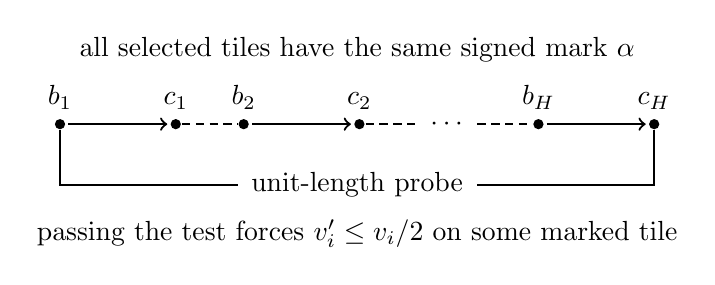
\begin{tikzpicture}[x=0.98cm,y=0.85cm,thick]
  \node at (3.85,1.12) {all selected tiles have the same signed mark \(\alpha\)};
  \foreach \x/\t in {0/{b_1},1.50/{c_1},2.38/{b_2},
                       3.88/{c_2},6.20/{b_H},7.70/{c_H}} {
      \fill (\x,0) circle (1.85pt);
      \node[above] at (\x,0.07) {\(\t\)};
  }
  \draw[->] (0.11,0)--(1.39,0);
  \draw[densely dashed] (1.58,0)--(2.30,0);
  \draw[->] (2.49,0)--(3.77,0);
  \draw[densely dashed] (3.96,0)--(4.62,0);
  \node at (5.01,0) {\(\cdots\)};
  \draw[densely dashed] (5.41,0)--(6.12,0);
  \draw[->] (6.31,0)--(7.59,0);
  \draw (0,-0.08)--(0,-0.91)--(7.70,-0.91)--(7.70,-0.08);
  \node[fill=white,inner xsep=5pt] at (3.85,-0.91)
          {unit-length probe};
  \node at (3.85,-1.64) {passing the test forces \(v'_i\le v_i/2\)
                              on some marked tile};
\end{tikzpicture}
\caption{Signed displacements add along tile arrows because each dashed
join identifies the two adjacent centers. The probe limits the distance
between the first and last centers. The inequality compares an altimeter
reading before and after imposing that endpoint constraint.}
\label{fig:marked-probe}
\end{figure}

Choose \(\delta>0\) sufficiently small that
\(4kH\delta C_W<\beta/2\); this uses only the already fixed stage
parameters. We show that \(\beta nN\) marks yield \(\Omega(n)\) probes.
In a group \(G\), put \(a=\lceil\delta l_G\rceil\). Suppose at least
\(2Ha\) remaining tiles have one fixed mark. Split that many into \(H\)
disjoint sets of size \(2a\). From the first set start with all its
tiles as reachable. If at least \(a\) tiles of one set are reachable,
their distinct output positions have sampler neighbors among all but
fewer than \(a\) of the next set's inputs. Thus at least \(a\) tiles of
every succeeding set are reachable, giving a chain of length \(H\)
and contradicting maximality. Summed over groups, stages, and \(2k\) marks,
the number left is at most
\[
                 4kH\delta C_W nN+o(n).
\]
The ceiling error is \(o(n)\) because \(\min_G l_G\to\infty\) and the total
list length is \(O(n)\) with all stage parameters fixed. Hence at least
\(\Omega(n)\) chains were purchased.

Consider any core-consistent sequence of grid arrays \(x\) with strictly
positive lower limit of the excess, and any sequence \(x'\) consistent
after purchasing those probes. The starting centers of the chains are
distinct roots. All but \(o(n)\) chains therefore admit the coordinate
assignment in Lemma~\ref{lem:protocol-local} at \(x'\). Write
\(v_i'=(x_i'-M)_+\). On each such chain at least one of its marking
coordinates satisfies \(v_i'\le v_i/2\). Otherwise, since \(s\le1\), each
tile would have displacement along the common mark at least
\[
                    T/(4\sqrt{k})-\eta>0 .
\]
Joins have equal coordinates on their two sides, so the sum of the
signed displacements is the signed endpoint displacement. By the choice of \(H\), it exceeds \(1+\eta\), contradicting the imposed probe.

To compare the resulting change in score with the probe fee, observe
that the divergence of $g(u)=(u-M)_+^2$ satisfies
\[
 g(u')-g(u)-g'(u)(u'-u)
        \ \ge\ \big((u'-M)_+-(u-M)_+\big)^2.
\]
This follows by considering the positions of $u$ and $u'$ relative to $M$.
For one of the changed coordinates on each good chain, this inequality
and the marking threshold give a contribution to
\((s/2)\mathcal D_f(x',x)\) of at least
\[
      \frac{sW^{-4}(v_i-v_i')^2}{2nNT^2}
                \ge \frac{W^{-4}}{32k nN}.
\]
The chosen coordinates are distinct, and every other contribution is
nonnegative. Each probe costs \( t^p/n\), which is at most
\(W^{-4}/(64k nN)\) once \(W\) is large enough, since
\(W^4 N t^p=O(W^4t^{p-1})\to0\). With \(\Omega(n)\) chains and only \(o(n)\)
exceptions, the lower limit of \((s/2)\mathcal D_f(x',x)-P\) is strictly
positive. This verifies the activation condition.

All requirements on \(W\) depend only on \(k\) and the initially fixed
protocol parameters. Fix such a \(W\), then the density \(\delta\), the
core-ball radius, \(M\) and \(c_0\), in that order. They are independent
of \(h,w\) and the permutation. Proposition~\ref{prop:adaptive-probing}
now supplies the exact protocols and budget in
Theorem~\ref{thm:protocol}.
